\documentclass[10pt,conference]{IEEEtran}
\let\labelindent\relax
\usepackage{enumitem}
\usepackage{graphicx}
\usepackage{cite}
\usepackage{url}

\title{Title}
\author{\IEEEauthorblockN{Chelsea Farley, Ryan Lewis, David Armstrong, Rina Gao and Ryunosuke Madenokoji}
\IEEEauthorblockA{The University of Auckland}}
\date{Today}

\begin{document}
\maketitle

\begin{abstract}
\end{abstract}

\section{Introduction}
There has been an increase in the overall traffic volume on the Web. The rate of increase of data traffic has been shown to follow Moore's law \cite{williams05}. Moore's law as it pertains to data traffic, states that the overall traffic volume will double annually. This property of data traffic means that the scalability of the Web is more important than ever. Additionally, the time an average user will wait for a page to load has decreased from eight seconds in 2000 to three seconds in 2009 \cite{Butkiewicz}. Therefore, it is becoming paramount that optimisations are made to improve Web performance.

In order to improve the performance and scalability of the Web, we must first develop an understanding of current Web workload characteristics and how they have changed over time. An understanding of the evolution of workload characteristics is vital in the development of effective caching architectures which, in turn, leads to improved performance. Additionally, workload analysis can aid in capacity planning, generating workload-generating models and network administration. Therefore, the purpose of this paper is to revisit several of the invariants identified by Arlitt and Williamson \cite{keynote} and evaluate whether they are applicable to a more recent Web server log. We will be analysing two of the Web server logs used in Arlitt and Williamson's original study: a departmental-level Web server at the University of Calgary and a campus-wide Web server at the University of Saskatchewan \cite{keynote}. Our more recent Web server log has data that was collected over a one year period between 2006 and 2007 from an academic conference Web site.

The remainder of the paper is organised as follows. In the following section we will discuss works related to our analysis and what our investigation contributes. In section \ref{methodology} we describe the characteristics we have chosen to analyse, and the metrics and tools we used to perform this study. Then we will explain the results we recorded in section \ref{results} and explain the practical implications of these results in section \ref{discussion}. Finally, we will conclude our paper and examine potential future work in the area of web workload characterisation in section \ref{conclusions}.

\section{Related Work}\label{related_work}
There have been several studies investigating the characteristics of Web workloads. These studies can be useful in understanding the evolution of Web traffic under differing conditions. In order to improve the scalability and performance of the Internet, we must have a complete understanding of the different traffic flows it may have to withstand. We have summarised several previous studies to provide an overview of these traffic flows. 

Arlitt and Jin \cite{world_cup} analysed data from the 1994 World Cup website. This study was motivated by the high volume of users accessing the site, and therefore the potential to extrapolate the future characteristics of web traffic. They discovered that most users are interested in cacheable files and thus caching plays an important role in the scalability and performance of the Internet. They also found that most user sessions had only one request per session, and therefore managing how connections are closed may be improved by examining session properties.

In 1996 and 1997, Arlitt and Williamson \cite{keynote, invariants} analysed logs from six Web servers and presented their findings. The motivation of their study was to find invariants of Web workload characteristics across six server logs. These invariants would be useful in the development of techniques for improving caching and the general performance of the Web. They found 10 invariants which may be useful in future analyses of Web traffic. They also discovered that there is the opportunity for caching to improve performance, and more specifically that caching to reduce the number of requests may be more effective than caching to reduce bytes transferred. 
This study was superseded by a study by Faber et al. \cite{Faber} which looked into the original ten invariants, but also discovered three more. Their study concludes that many of the original ten invariants have remained relatively the same in the twenty years that have passed. Among the three new invariants discovered, one showed a significant difference in results between scientific and general websites.

Williams et al. \cite{williams05} produced an analysis of Web server logs from 2004 from the same three universities as the initial paper \cite{keynote}. The aim of the analysis was to uncover the impact of Moore's law on the ten invariants of the initial study. They concluded that despite the increase in traffic volume, most of the ten invariants remained unchanged. However, the percentage of successful requests and the percentage of HTML and image files transferred had decreased. 

In 2007, Gill et al. \cite{youtube} analysed YouTube usage on the University of Calgary network and collected statistics on global video popularity. The aim of this study was to investigate Web 2.0 workload characteristics to allow for improvements in network management, capacity planning and the design of new systems. Web 2.0 marks a shift towards user generated content and with it comes a plethora of metadata. It was found that although the concentration of references was reduced from that of traditional Web workloads \cite{keynote}, metadata should be used to improve the effectiveness of caching.

Cherkasova and Gupta \cite{Cherkasova} investigated client access patterns, media server access trends, and the evolution of media on websites over time. Their research was split into static and temporal analysis of the data. They looked at the locality of accesses, which was similar to that of a Web server with 14\%-30\% of the server files accounting for 90\% of media sessions, and 92\%-94\% of the bytes transferred. Additionally, 16\%-19\% of files were accessed only once, and the first five weeks of a file’s existence account for 70\%-80\% of its total accesses. They also looked into the trends associated with media session lengths, and the behavior of clients with incomplete sessions. Their research concentrated on comparing media server workloads with traditional web server workloads.

In 2002, Bai and Williamson \cite{Bai} analysed the request arrival rate at each level of a multi-layer web proxy caching hierarchy using trace-driven simulation and artificial web workloads. The presence of a Web proxy cache means that requests are removed from the Web server request stream when there is a cache hit at the proxy. The results showed that there was a decrease in the peak and mean request arrival rates in the presence of a multi-layer web caching hierarchy. However, they also noted that the burstiness of request arrivals may vary or stay the same. They discovered that a gamma distribution may be used to model the arrival of requests in a web caching hierarchy.

Almeida et al. \cite{almeida} analysed the performance of a PC acting as dedicated Web server. The purpose of their study was to measure the activity and resource consumption of the operating system using WebMonitor. This provided insight into variances in the performance of servicing web requests. They observed similar user session properties to Arlitt and Jin \cite{world_cup} as most requests required a new connection, which may be problematic for operating systems that are not designed to cope with this. This highlighted the importance of operating system and network protocol implementation.

Almeida et al. \cite{reference_locality} examined models for gathering data on spatial and temporal locality. The motivation of this study was the insufficiency of simple popularity based models being insufficient for capturing spatial and temporal locality. They discovered that for accesses following a temporal access pattern, caching is beneficial in improving performance. Whereas, for accesses following a spatial access pattern, prefetching is beneficial in improving performance.

In 2012, Tantithamthavorn and Rungsawang \cite{facebook} conducted a study on Facebook usage at Kasetsart University based on a Web traffic log. Their study analysed the time spent communicating online, distribution of HTTP requests, Facebook traffic workload analysis, and more. The results showed that the distribution of HTTP Requests at the level of hostname followed a Zipfian distribution. Additionally, they suggested that long running sessions may be due to idle users. Overall the study showed a typical Web workload at a university.

\section{Methodology}\label{methodology}
\subsection{Characteristics}\label{lab:characteristics}
In this study, we have chosen to examine five of the characteristics identified by Arlitt and Williamson \cite{keynote}: the success rate, file types, file size distribution, one time referencing, and the concentration of references. We also look into two of the invariants found by Faber et al. \cite{Faber}: weekday versus weekend usage and diurnal usage. Finally, we add two original invariants: cache rate, and the effectiveness of caching.

The success rate looks at the occurrence of successful, found, and not modified status codes on requests to each of the three web servers. Size distribution examines the trend in the sizes of files on each of the three data sets. One time referencing looks at the percentage of files and bytes that are requested only once in the logged period, while the concentration of references is a measurement of the frequency of distinct file accesses. We compare the usage of these sites between weekdays and weekends, and also between daytime and nighttime. Cache rate looks at the ratio of number of accesses of a file, and the number of times it was cached, while the effectiveness of caching refers to the amount of bandwidth saved with caching.

\subsection{Metrics}
To determine which characteristics from section \ref{lab:characteristics} were present we decided on the following metrics:
\begin{itemize}[noitemsep]
    \item Unique IP addresses
    \item Number of times each status code appears
    \item Number of times each file is accessed
    \item Number of bytes saved via caching
    \item Number of bytes transferred
    \item The time each file is requested
\end{itemize}

\subsection{Unique IP Addresses}
Unique IP addresses is a count of how many unique IP addressess accessed each site. This metric allowed us to give an estimate of how many people were accessing the website. 

\subsection{Number of times each status code appears}
We recorded a count of each status code or range of status codes so that we could characterise both success rate and caching.
The number of successful requests is the total number of requests that had the status code of either 2xx (Success) or 3xx (Redirection). This allows us to characterise the workloads based on percentage of successful requests.
We also were able to see how many requests were cached by the client based on the count of 304 (Not Modified) status codes in the logs. Counting the number of 304 statuses compared to the total number of requests allows us to characterize the effectiveness of caching on number of requests.

\subsection{Number of times each file is accessed}
This metric is a count of each access to a particular resource.
This measurements of this metric show how concentrated the requests are in terms of which files are the most popular and would benefit from higher availablility. In addition this metric will show the number of files accessed only a single time.

\subsection{Number of bytes transferred}
This metric gathers the size of each file that is transferred. We used it to calculate the mean and median size for each request. 
It also allowed us to calculate the bandwidth savings from client side caching by combining this metric with the status codes collected.

\subsection{Number of bytes transferred}
This metric simply totalled up the total bandwidth used over the logging period. It allowed us to see the relative effect of caching when comparing the two datasets of different sizes.

\subsection{The time each file is accessed}
We also recorded the time of each file access binned into hourly bins. This metric allowed us to plot the number of accesses over time to see if the workload is still following a diurnal pattern. It also allowed for comparison between the weekday and weekend workload.

\subsection{Tools}
To record the results we used a custom parser written in python. By custom writing the parser it allowed for rapid development as there was no confusion about the abilities of the tool. It was also possible to add measurements to the tool no learning curve, which was necessary due to the limited timeframe of this research.

\section{Results}\label{results}

\begin{figure}
    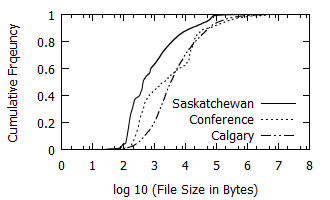
\includegraphics{images/filesize}
    \caption{Hi}\label{fig:filesize}
\end{figure}

\begin{figure}
    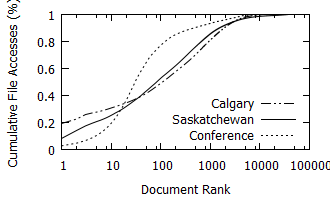
\includegraphics{images/concentration}
    \caption{Hi}\label{fig:file_accesses}
\end{figure}

\begin{figure*}
    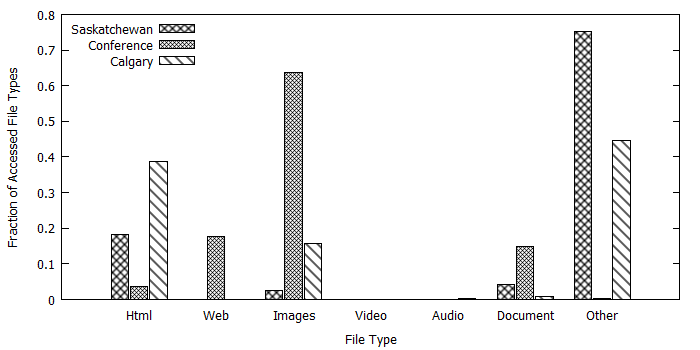
\includegraphics{images/filetype}
    \caption{Hi}\label{fig:file_types}
\end{figure*}

\subsection{Document Types}\label{sub:doc_types}
We decided to analyse the number of times different file types were accessed and present these as a fraction of the total number of file accesses. We categorised files into HTML, images, web, video, audio, document and other. We defined the web category as files with the extensions \texttt{.css}, \texttt{.js}, \texttt{.cfm}, \texttt{.php}, \texttt{.asp}, \texttt{.aspx} and \texttt{.xml}. We also defined other as any files which were of an unknown type. We expected this to be useful characteristic to analyse as it allows us to see trends in what files are being accessed. The results of this analysis across all three Web servers are shown in Figure \ref{fig:file_types}.

The document type analysis revealed an interesting difference between the more 2006-2007 log and the 1994-1995 logs. We can see that in the 1994-1995 logs, HTML were the most accessed documents excluding documents of an unknown type. This observation is consistent with results obtained by Arlitt and Williamson \cite{keynote}. However, we can see that in the 2006-2007 log only a small fraction of the files accessed were HTML files. We can also note that in the 2006-2007 log, there were substantially more requests for images and Web file types than in the 1994-1995 logs. We have attributed this to increasing network bandwidth and advancements in the technology available for Web development.

\section{Discussion}\label{discussion}

\section{Conclusions and Future Work}\label{conclusions}

\bibliographystyle{IEEEtran}
\bibliography{references.bib}
\end{document}